\chapter{Lecture}\label{part2:lec10} %%% 10
\markboth{\thechapter. Lecture}{\thechapter. Lecture}

Let\pageoriginale us recapitulate the formulae we has last time.

\begin{align*}
  \mathscr{V}_1 (\mathscr{V}, q) & = \frac{1}{i} \sum^\infty_{n=-
    \infty} (-)^n q^{\left( \frac{2n+1}{2}\right)^2} e^{(2n+1)\pi i
    \mathscr{V}}\\
  & = 2\sum^\infty_{n= \infty} (-)^n q^{\left(\frac{2n+1}{2}\right)^2} 
  \sin(2n+1) \pi \mathscr{V}\\
  & = 2 q^{1/4} \sin \pi \mathscr{V} \prod^\infty_{m=1} \left(1-
  q^{2m}\right)\left(1-q^{2m} e^{2 \pi i \mathscr{V}}\right)\left(1-
  q^{2m} e^{- 2 \pi i \mathscr{V}}\right) \tag{1}\label{part2:lec10:eq1}\\
  \mathscr{V}_2 (\mathscr{V}, q) & = \sum^\infty_{n=-
    \infty} q^{\left( \frac{2n+1}{2}\right)^2} e^{(2n+1)\pi i
    \mathscr{V}}\\
  & = 2\sum^\infty_{n= 0} q^{\left(\frac{2n+1}{2}\right)^2} 
  \cos(2n+1) \pi \mathscr{V}\\
  & = 2 q^{1/4} \cos \pi \mathscr{V} \prod^\infty_{m=1} \left(1-
  q^{2m}\right)\left(1+q^{2m} e^{2 \pi i \mathscr{V}}\right)\left(1+
  q^{2m} e^{- 2 \pi i \mathscr{V}}\right) \tag{2}\label{part2:lec10:eq2}\\  
  \mathscr{V}_3 (\mathscr{V}, q) & = \sum^\infty_{n=-
    \infty} q^{n^2} e^{2 \pi i \mathscr{V}}\\
  & = 1+2 \sum^\infty_{n= 1} q^{n^2} \cos 2n \pi \mathscr{V}\\
  & = \prod^\infty_{m=1} \left(1-
  q^{2m}\right) \left(1+q^{2m-1} e^{2 \pi i \mathscr{V}}\right)\left(1+
  q^{2m-1} e^{-2 \pi i \mathscr{V}}\right) \tag{3}\label{part2:lec10:eq3}\\
  \mathscr{V}_4 (\mathscr{V}, q) &= \sum^\infty_{n=-\infty} (-)^n
  q^{n^2} e^{2n \pi i \mathscr{V}}\\
  & = 1+ 2 \sum^\infty_{n=1} (-)^n q^{n^2} \cos 2n \pi \mathscr{V}\\
  & = \prod^\infty_{m=1} (1-q^{2m})(1- q^{2m-1}e^{2 \pi i
    \mathscr{V}})(1-q^{2m-1}e^{-2 \pi i \mathscr{V}}) \tag{4}\label{part2:lec10:eq4}
\end{align*}

We\pageoriginale started with $\mathscr{V}_3$ and shifted the
argument $\mathscr{V}$ by `periods', and we had, writing $q= e^{\pi i
  \tau}$, 
\begin{equation*}
  \begin{aligned}
    \mathscr{V}_3 (\mathscr{V}+ 1, q) & = \mathscr{V}_3 (\mathscr{V},
    q)\\
    \mathscr{V}_3 (\mathscr{V}+\tau, q)& = q^{-1} e^{-2 \pi i
      \mathscr{V}} \mathscr{V}_3 (\mathscr{V}, q).
  \end{aligned}\tag{5}\label{part2:lec10:eq5}
\end{equation*}

Then we took `half-periods' and then something new happened, and we
gave names to the new functions:
\begin{equation*}
  \begin{aligned}
    \mathscr{V}_3 \left(\mathscr{V}+ \frac{1}{2}, q\right) & =
    \mathscr{V}_4 (\mathscr{V}, q)\\
    \mathscr{V}_3 \left(\mathscr{V}+ \frac{\tau}{2}, q\right) & =
    q^{-1/4} e^{-2 \pi i \mathscr{V}} \mathscr{V}_2 (\mathscr{V}, q)\\
    \mathscr{V}_3 \left(\mathscr{V}+ \frac{1+\tau}{2}, q\right) & =
    i q^{-1/4} e^{- \pi i \mathscr{V}} \mathscr{V}_1 (\mathscr{V}, q)    
  \end{aligned}\tag{6}\label{part2:lec10:eq6}
\end{equation*}

Let us study how these functions alter when the argument $\mathscr{V}$
is changed by 1, $\tau$, $1/2$, $\tau/2$, $(1+
\tau)/2$. $\mathscr{V}\to \mathscr{V}+1$ is trivial; $\mathscr{V}\to
\mathscr{V}+1/2$ is also easy to see by inspection. Let us take
$\mathscr{V}+\tau$. (We suppress the argument $q$ for convenience of
writing). 
\begin{align*}
  \mathscr{V}_1 (\mathscr{V}) &= \frac{1}{i} q^{1/4} e^{2 \pi i
    \mathscr{V}} \mathscr{V}_3 \left(\mathscr{V}+ \frac{1+ \tau}{2}
  \right)\\
  \therefore \quad  \mathscr{V}_1 (\mathscr{V}+ \tau) & = \frac{1}{i}
  q^{1/4} e^{\pi i (\mathscr{V} + \tau)} \mathscr{V}_3 \left(\mathscr{V}+
  \tau+ \frac{1+\tau}{2}\right)\\
  & = \frac{1}{i} q^{1/4} e^{\pi i \mathscr{V}} q q^{-1} e^{- 2 \pi
    i(\mathscr{V}+1+ \tau/2)} \mathscr{V}_3 \left(\mathscr{V}+
  \frac{1+\tau}{2}\right)\\
  & = e^{-2 \pi i \mathscr{V}} e^{-\pi i (1+ \tau)} \mathscr{V}_1
  (\mathscr{V}, q)\\
  & = -A \mathscr{V}_1 (\mathscr{V}, q),
\end{align*}
where\pageoriginale $A= q^{-1} e^{-2 \pi i \mathscr{V}}$; the other conspicuous
factor which occurs in similar contexts is denoted $B= q^{-1/4} e^{-2
  \pi i \mathscr{V}}$.

The other transformations can be worked out in a similar way by first
going over to $\mathscr{V}_3$. We collect the results below in tabular
form. 

\medskip
\tabcolsep=10pt
\setlength\extrarowheight{5pt}
\begin{tabular}{||>{$}c<{$}||>{$}c<{$}||>{$}c<{$}||>{$}c<{$}||>{$}c<{$}||>{$}c<{$}||}
  \hhline{|t:======:t|}
  & \mathscr{V}+1 & \mathscr{V}+ \tau & \mathscr{V}+ \frac{1}{2} &
  \mathscr{V}+\frac{3}{2} & \mathscr{V}+ \frac{1+\tau}{2}\\[5pt]
  \hhline{|:======:|}
  \mathscr{V}_1 & -\mathscr{V}_1 & -A\mathscr{V}_1 & \mathscr{V}_2 & i
  B \mathscr{V}_4 & B \mathscr{V}_3\\[5pt]
  \hhline{|:======:|}
  \mathscr{V}_2 & -\mathscr{V}_2 & A\mathscr{V}_2 & -\mathscr{V}_1 & 
  B \mathscr{V}_3 & -i B \mathscr{V}_4\\[5pt]
  \hhline{|:======:|}  
  \mathscr{V}_3 & \mathscr{V}_3 & A\mathscr{V}_3 & \mathscr{V}_4 & 
  B \mathscr{V}_2 & B \mathscr{V}_1\\[5pt]
  \hhline{|:======:|}  
  \mathscr{V}_4 & \mathscr{V}_4 & -A\mathscr{V}_4 & \mathscr{V}_3 & i
  B \mathscr{V}_1 & B \mathscr{V}_2\\[5pt]
  \hhline{|b:======:b|}   
\end{tabular}
\medskip

It may be noticed that each column in the table contains all the four
functions; so does each now.

The systematique of the notation for the $\mathscr{V}$-functions is
rather questionable. Whittaker and Watson write $\mathscr{V}$ instead
of $\pi \mathscr{V}$, which has the unpleasant consequence that the
`periods' are then $\pi$ and $\pi \tau$. Our\pageoriginale notation
is the same as in Tannery and Molk. An attempt was made by Kronecker
to systematise a little the unsystematic notation. Charles Hermite
introduced the following notation:
\begin{align*}
  \mathscr{V}_{\mu \nu} (\mathscr{V}, q) & = \sum^\infty_{n=-\infty}
  (-)^{\nu n} q^{\left( \frac{2r+ \mu}{2} \right)^2} e^{(2n+ \mu) \pi
    i \mathscr{V}}\\
  & = \sum^\infty_{n=- \infty} (-)^{\nu n} e^{\left(\frac{2n+\mu}{2}
    \right)^2 \pi i \tau} e^{(2n+\mu) \pi i \mathscr{V}}
\end{align*}
where $\mu, \nu=0,1*****$. In this notation, 
\begin{align*}
  \mathscr{V}_{00} (\mathscr{V}, q) & = \mathscr{V}_3(\mathscr{V},
  q)\\
  \mathscr{V}_{01} (\mathscr{V}, q) & = \mathscr{V}_4 (\mathscr{V},
  q)\\
  \mathscr{V}_{10} (\mathscr{V}, q) & = \mathscr{V}_2 (\mathscr{V},
  q)\\ 
  \mathscr{V}_{11} (\mathscr{V}, q) & = i \mathscr{V}_1(\mathscr{V}, q).
\end{align*}

This, however, has not found any followers.

While writing down derivatives, we always retain the convention that a
prime refers to differentiation with respect to $\mathscr{V}$:
$$
\mathscr{V}'_\alpha (\mathscr{V}, q) = \frac{\partial}{\partial \nu}
\mathscr{V}_\alpha (\mathscr{V}, q) ~(\alpha=1, 2, 3, 4)
$$

Taking partial derivatives, we have
\begin{align*}
  \frac{\partial}{\partial \tau} \mathscr{V}_{\mu \nu}
  (\mathscr{V}/\tau) & = \sum^\infty_{n=- \infty} (-)^{\nu n} \pi i
  \left(\frac{2n+ \mu}{2}\right) e^{\left(\frac{2n+\mu}{2}\right)^2
    \pi i \tau} e^{(2n + \mu)\pi i \mathscr{V}},\\
    \text{and} \qquad   \frac{\partial^2}{\partial \mathscr{V}^2}
    \mathscr{V}_{\mu \nu} 
  (\mathscr{V}/\tau) & = \sum^\infty_{n=- \infty}(-)^{\nu n} 
  e^{\left(\frac{2n+ \mu}{2}\right)^2 \pi i \tau} \pi^2 i^2 (2n +
  \mu)^2 e^{(2n +\mu)\pi i \mathscr{V}},\qquad 
\end{align*}

Comparing\pageoriginale  these we see that they agree to some extent;
in fact,
\begin{equation*}
  4 \pi i \frac{\partial}{\partial \tau} \mathscr{V}_{\mu \nu}
  (\mathscr{V}/\tau)= \frac{\partial^2}{\partial \nu^2}
  \mathscr{V}_{\mu \nu} (\mathscr{V}/\tau) \tag{7}\label{part2:lec10:eq7}
\end{equation*}

This is a partial differential equation of the
second order, a parabolic equation with constant coefficients. It is
fundamental to write $i \tau=- t$; (\ref{part2:lec10:eq7}) then becomes the differential
equation for heat conduction. $\mathscr{V}$-functions are thus very
useful tools in applied mathematics; they were used by Poisson and
Fourier in this connection. 

Again, 
\begin{align*}
  \frac{\partial}{\partial q} \mathscr{V}_{\mu \nu}
  (\mathscr{V}, q) & = \sum^\infty_{n=- \infty} (-)^{\nu} 
  \left(\frac{2n+ \mu}{2}\right)^2 q^{\left(\frac{2n+\mu}{2}\right)^2
    -1} e^{(2n+\mu) \pi i \mathscr{V}},\\ 
  & - 4 \pi^2 q \frac{\partial}{\partial q} \mathscr{V}_{\mu \nu}
  (\mathscr{V}, q)= \frac{\partial^2}{\partial \nu^2} \mathscr{V}_{\mu
    \nu} (\mathscr{V}, q), \tag{8}
\end{align*}
which is another form of (\ref{part2:lec10:eq7}). Here the uniformity
of notation was 
helpful; it was not necessary to discuss the different functions
separately.

We now pass on to another important topic. The zeros of the
theta - functions.

The $\mathscr{V}$-functions are more or less periodic. The exponential
factor that is picked up on passing from one parallelogram to another
is non-zero and can accumulate. It is evident from the definition that 
$$
\mathscr{V}, (0, q)=0.
$$

On\pageoriginale the other hand $\mathscr{V}_2$, $\mathscr{V}_3$, $\mathscr{V}_4\neq
0$. (when the argument $\mathscr{V}$ is 0 we write hereafter simply
$\mathscr{V}$). This is so because the infinite products are
absolutely convergent. (Let us recall that a product like $1 \cdot
\frac{1}{2} \cdot \frac{1}{3} \cdots$ is not properly convergent in
the product sense). Again from the definitions,
\begin{align*}
  \mathscr{V}_2 \left(\frac{1}{2}\right) & =0\\
  \mathscr{V}_3 \left(\frac{1+\tau}{2}\right) & =0\\  
  \mathscr{V}_4 \left(\frac{\tau}{2}\right) & =0
\end{align*}

So far we have one zero per parallelogram for each of the functions;
and there can be no other in a parallelogram, as can be seen from the
infinite product expansions. The zeros of $\mathscr{V}_1 (\mathscr{V},
q)$ are $m_1 + m_2 \tau (m_1, m_2$ integers), for $1- e^{2 \pi i m
  \tau}e^{2 \pi i \mathscr{V}}=0$ implies $m \tau + \mathscr{V}_1 =
m_1$ or $\mathscr{V}= m_1 - m \tau$. The zeros of $\mathscr{V}_1
(\mathscr{V}, q), \mathscr{V}_2(\mathscr{V}, q),
\mathscr{V}_3(\mathscr{V}, q), \mathscr{V}_4 (\mathscr{V}, q)$ in the
fundamental parallelogram are nicely arranged in order at the points
$0, \frac{1}{2}, \frac{1+\tau}{2}, \frac{\tau}{2}$ respectively.  

\begin{figure}[H]
\centering{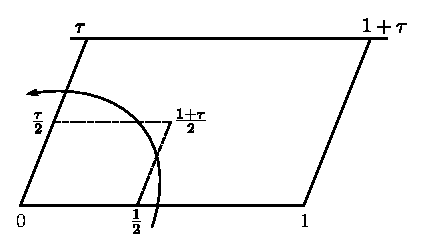
\includegraphics{vol2-figures/fig2.13.eps}}
\end{figure}

All\pageoriginale the zeros are therefore given by the formulae:
\begin{align*}
  \mathscr{V}_1 (m_1+ m_2 \tau) & = 0\\
  \mathscr{V}_2 \left(m_1+m_2 \tau + \frac{1}{2}\right)& =0\\
  \mathscr{V}_3 \left(m_1+m_2 \tau + \frac{1+\tau}{2}\right)& =0\\
  \mathscr{V}_4 \left(m_1+m_2 \tau + \frac{\tau}{2}\right)& =0
\end{align*}

It is of interest to study $\mathscr{V}_\alpha (0, q)$ (usually
written $\mathscr{V}_\alpha$).
\begin{align*}
  \mathscr{V}_1 (0) & =0 \\
  \mathscr{V}_2(0) & =\sum^\infty_{n=-\infty} q^{\left(2n+
    \frac{1}{2}\right)^2}\\
  & = 2 q^{1/4} \prod^\infty_{m=1} (1- q^{2m})(1+q^{2m})^2\\
  & = \mathscr{V}_2\\
  \mathscr{V}_3 (0) & = \sum^\infty_{n=-\infty} q^{n^2}\\
  & = \prod^\infty_{m=1} (1- q^{2m})(1+ q^{2m-1})\\
  \mathscr{V}_4(0) & = \sum^\infty_{n=-\infty} (-)^n q^{n^2}\\
  & = \prod^\infty_{m=1} (1- q^{2m})(1-q^{2m-1})^2
\end{align*}

We\pageoriginale cannot anything of interest in $\mathscr{V}_1$. Let
us look at the others.
\begin{align*}
  \mathscr{V}'_1 (0, q) & = \mathscr{V}'_1= 2 \pi \sum^\infty_{n=0}
  (-)^n (2n+1)q^{\left(\frac{2n+1}{2}\right)^2}\\
  & = 2 q^{1/4} \left[ \pi \cos \pi \mathscr{V} \prod^\infty_{m=1}
    (\cdots) + \sin \pi \mathscr{V} \left(\prod^\infty_{m=1}(\cdots)
    \right)' \right]_{\mathscr{V}=0}\\
  & = 2 \pi q^{1/4} \prod^\infty_{m=1} (1- q^{2m})^3
\end{align*}

Immediately we see that this yields the interesting identity of
Jacobi.
$$
\prod^\infty_{m=1} (1- q^{2m})^3 = \sum^\infty_{n=0} (-)^n (2n+1)q^{n^2+n},
$$
or, replacing $q^2$ by $x$,
$$
\prod^\infty_{n=1} (1- x^n)^3 = \sum^\infty_{n=0} (-)^n (2n+1) x^{n(n+1)/2}
$$

We had proved this earlier by the method of formal power series. Here
we can differentiate with good conscience. 

Now
\begin{align*}
  \pi \mathscr{V}_2 \mathscr{V}_3 \mathscr{V}_4 & = \mathscr{V}_1'
  \left( \prod^\infty_{m=1} (1+ q^{2m}) (1+
  q^{2m-1})(1-q^{2m-1})\right)^2\\
  & = \mathscr{V}_1' \left( \prod^\infty_{m=1} (1+q^{2m})(1-q^{4m-2})\right)^2,
\end{align*}
which\pageoriginale becomes, on replacing $q^2$ by $x$,
$$
\mathscr{V}_1' \left[ \prod^\infty_{m=1} (1+ x^n)\left(1-x^{2n-1}\right)\right]^2
$$ 

However, $\prod\limits^\infty_{m=1} (1+x^n)(1-x^{2n-1})=1$. We
therefore have the very useful and pleasant formula
$$
\mathscr{V}'_1 = \pi \mathscr{V}_2 \mathscr{V}_3 \mathscr{V}_4
$$
